%==============================================================================
% Chapitre 57 - Les chokes
%==============================================================================

\section{Introduction}

Les chokes sont des dispositifs destinés à modifier la dispersion des
projectiles dans les armes à canon lisse.

Ils jouent un rôle important dans les performances des fusils de chasse.

Leur influence est particulièrement visible avec les cartouches à grenaille.

\begin{aretenir}

Un choke modifie la dispersion de la gerbe en agissant sur la sortie de la
charge à la bouche du canon.

\end{aretenir}

\section{Principe général}

Un choke correspond à un léger rétrécissement situé à l'extrémité du canon.

Ce rétrécissement agit sur la charge lors de son passage.

L'objectif recherché est généralement de contrôler la dispersion de la gerbe.

\begin{figure}[htbp]
\centering

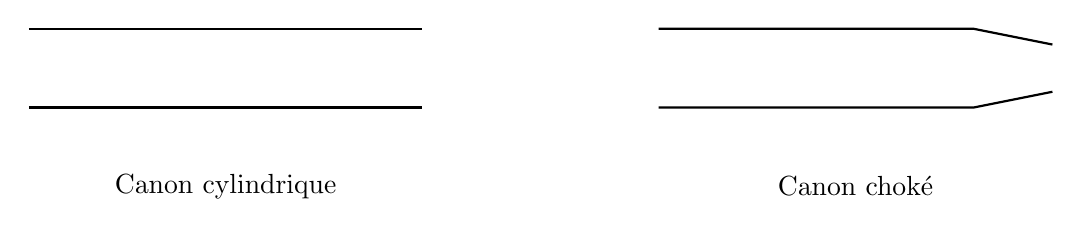
\begin{tikzpicture}[scale=1]

% Canon cylindrique
\draw[thick] (0,1) -- (5,1);
\draw[thick] (0,0) -- (5,0);

\node at (2.5,-1)
{Canon cylindrique};

% Canon choké
\begin{scope}[xshift=8cm]

\draw[thick]
(0,1)
--
(4,1)
--
(5,0.8);

\draw[thick]
(0,0)
--
(4,0)
--
(5,0.2);

\node at (2.5,-1)
{Canon choké};

\end{scope}

\end{tikzpicture}

\caption{Principe simplifié d'un choke placé à l'extrémité du canon.}
\label{fig:principe_choke}

\end{figure}

\section{Pourquoi utiliser un choke ?}

Selon les situations de chasse, il peut être souhaitable d'obtenir :

\begin{itemize}
    \item une gerbe large ;
    \item une gerbe intermédiaire ;
    \item une gerbe dense.
\end{itemize}

Les chokes permettent d'adapter le comportement du fusil à l'usage recherché.

\section{Canon cylindrique}

Un canon cylindrique ne comporte pratiquement aucun rétrécissement.

La dispersion obtenue est généralement importante.

Cette configuration est souvent adaptée aux tirs à courte distance.

\section{Quart de choke}

Le quart de choke constitue un léger rétrécissement.

Il réduit modérément la dispersion.

\section{Demi-choke}

Le demi-choke représente un compromis très répandu.

Il offre un équilibre entre ouverture de la gerbe et concentration.

\section{Trois-quarts de choke}

Le trois-quarts de choke produit une gerbe généralement plus dense.

Il est souvent utilisé pour des tirs plus éloignés.

\section{Full choke}

Le full choke correspond à un rétrécissement plus important.

Il permet généralement d'obtenir la gerbe la plus concentrée parmi les
configurations classiques.

\begin{figure}[htbp]
\centering

\begin{tikzpicture}[scale=0.9]

% Cylindrique
\draw (0,1) -- (3,1);
\draw (0,0) -- (3,0);
\node at (1.5,-0.8) {Cyl.};

% 1/4
\begin{scope}[xshift=4cm]
\draw (0,1) -- (2.5,1) -- (3,0.9);
\draw (0,0) -- (2.5,0) -- (3,0.1);
\node at (1.5,-0.8) {1/4};
\end{scope}

% 1/2
\begin{scope}[xshift=8cm]
\draw (0,1) -- (2.2,1) -- (3,0.8);
\draw (0,0) -- (2.2,0) -- (3,0.2);
\node at (1.5,-0.8) {1/2};
\end{scope}

% 3/4
\begin{scope}[xshift=12cm]
\draw (0,1) -- (2,1) -- (3,0.7);
\draw (0,0) -- (2,0) -- (3,0.3);
\node at (1.5,-0.8) {3/4};
\end{scope}

% Full
\begin{scope}[xshift=16cm]
\draw (0,1) -- (1.8,1) -- (3,0.6);
\draw (0,0) -- (1.8,0) -- (3,0.4);
\node at (1.5,-0.8) {Full};
\end{scope}

\end{tikzpicture}

\caption{Illustration simplifiée des principaux niveaux de choke.}
\label{fig:niveaux_choke}

\end{figure}

\section{Influence sur la gerbe}

Lorsque le choke augmente :

\begin{itemize}
    \item la dispersion diminue ;
    \item la densité de la gerbe augmente ;
    \item la portée utile tend à augmenter.
\end{itemize}

\begin{figure}[htbp]
\centering

\begin{tikzpicture}

% Gerbe ouverte
\draw[dashed] (0,0) circle (2);

\foreach \x/\y in {
-1.3/0.7,-1.1/-0.5,-0.5/1.2,
0.4/1.0,1.2/0.6,1.0/-0.8,
0.0/0.0,-0.3/-1.2,0.6/-1.1,
-1.5/0.0,1.4/0.1
}
{
\fill (\x,\y) circle (0.06);
}

\node at (0,-3)
{Canon cylindrique};

% Gerbe dense
\begin{scope}[xshift=8cm]

\draw[dashed] (0,0) circle (2);

\foreach \x/\y in {
-0.5/0.4,-0.3/0.6,-0.1/0.2,
0.2/0.5,0.5/0.2,
-0.4/-0.3,-0.1/-0.5,
0.2/-0.4,0.5/-0.2,
0.0/0.0,0.1/0.1,
-0.2/0.1
}
{
\fill (\x,\y) circle (0.06);
}

\node at (0,-3)
{Full choke};

\end{scope}

\end{tikzpicture}

\caption{Influence simplifiée du choke sur la densité de la gerbe.}
\label{fig:gerbe_choke}

\end{figure}

\section{Distance de tir}

Le choix du choke dépend fortement de la distance prévue.

Un choke très serré peut être peu adapté à un tir très rapproché.

Inversement, un choke très ouvert peut devenir insuffisant à longue distance.

\section{Compatibilité avec les munitions}

Toutes les munitions ne réagissent pas de la même manière.

Le comportement dépend notamment :

\begin{itemize}
    \item de la grenaille ;
    \item de la bourre ;
    \item de la vitesse ;
    \item du diamètre des projectiles.
\end{itemize}

\section{Influence de la bourre}

La bourre et le choke agissent conjointement.

Le résultat final dépend de l'interaction entre ces deux éléments.

\section{Chokes fixes}

Pendant longtemps, les fusils utilisaient des chokes fixes usinés directement
dans le canon.

Le choix était alors permanent.

\section{Chokes interchangeables}

De nombreux fusils modernes utilisent des chokes démontables.

Cette solution offre davantage de flexibilité.

\begin{figure}[htbp]
\centering

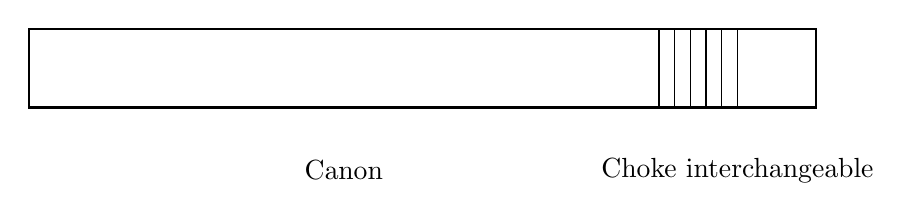
\begin{tikzpicture}[scale=1]

% Canon
\draw[thick]
(0,0)
rectangle
(8,1);

% Choke
\draw[thick]
(8,0)
rectangle
(10,1);

% Filetage simplifié
\foreach \x in {8.2,8.4,8.6,8.8,9.0}
{
\draw (\x,0) -- (\x,1);
}

\node at (4,-0.8)
{Canon};

\node at (9,-0.8)
{Choke interchangeable};

\end{tikzpicture}

\caption{Exemple simplifié d'un choke interchangeable vissé à l'extrémité du canon.}
\label{fig:choke_interchangeable}

\end{figure}

\section{Choix pratique}

Le choix d'un choke dépend :

\begin{itemize}
    \item du type de chasse ;
    \item de la distance habituelle ;
    \item des munitions utilisées ;
    \item des préférences du tireur.
\end{itemize}

\section{Essais en cible}

Les résultats théoriques ne remplacent jamais les essais pratiques.

Les tirs sur cible permettent de vérifier la qualité réelle des gerbes.

\section{Idées reçues}

Les performances observées ne dépendent pas uniquement du choke.

Deux fusils équipés du même choke peuvent produire des résultats différents.

\section{Vers l'étude des gerbes}

Le choke constitue l'un des principaux moyens de contrôler la dispersion.

Le chapitre suivant examinera plus en détail la formation et l'analyse des
gerbes de grenaille.

\begin{figure}[htbp]
\centering

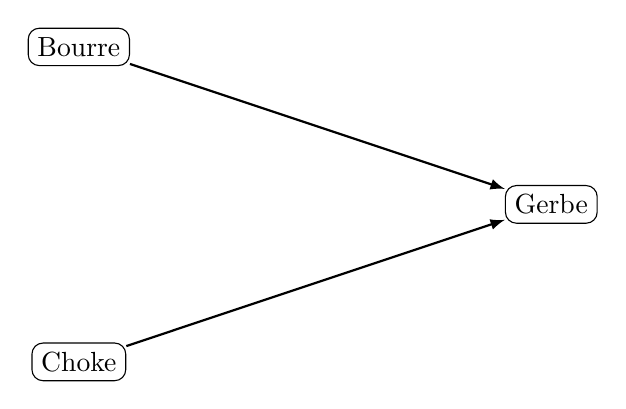
\begin{tikzpicture}[scale=1]

\node[draw,rounded corners]
(B)
at (0,2)
{Bourre};

\node[draw,rounded corners]
(C)
at (0,-2)
{Choke};

\node[draw,rounded corners]
(G)
at (6,0)
{Gerbe};

\draw[-latex,thick]
(B)
--
(G);

\draw[-latex,thick]
(C)
--
(G);

\end{tikzpicture}

\caption{La qualité de la gerbe dépend à la fois de la bourre et du choke.}
\label{fig:bourre_choke}

\end{figure}

\section{À retenir}

\begin{aretenir}

\begin{itemize}
    \item Un choke est un rétrécissement situé à l'extrémité du canon.
    \item Il permet de contrôler la dispersion de la gerbe.
    \item Plus le choke est important, plus la gerbe est généralement dense.
    \item Le comportement dépend également des munitions utilisées.
    \item Les essais en cible restent indispensables.
\end{itemize}

\end{aretenir}
